\documentclass[1p]{elsarticle_modified}
%\bibliographystyle{elsarticle-num}

%\usepackage[colorlinks]{hyperref}
%\usepackage{abbrmath_seonhwa} %\Abb, \Ascr, \Acal ,\Abf, \Afrak
\usepackage{amsfonts}
\usepackage{amssymb}
\usepackage{amsmath}
\usepackage{amsthm}
\usepackage{scalefnt}
\usepackage{amsbsy}
\usepackage{kotex}
\usepackage{caption}
\usepackage{subfig}
\usepackage{color}
\usepackage{graphicx}
\usepackage{xcolor} %% white, black, red, green, blue, cyan, magenta, yellow
\usepackage{float}
\usepackage{setspace}
\usepackage{hyperref}

\usepackage{tikz}
\usetikzlibrary{arrows}

\usepackage{multirow}
\usepackage{array} % fixed length table
\usepackage{hhline}

%%%%%%%%%%%%%%%%%%%%%
\makeatletter
\renewcommand*\env@matrix[1][\arraystretch]{%
	\edef\arraystretch{#1}%
	\hskip -\arraycolsep
	\let\@ifnextchar\new@ifnextchar
	\array{*\c@MaxMatrixCols c}}
\makeatother %https://tex.stackexchange.com/questions/14071/how-can-i-increase-the-line-spacing-in-a-matrix
%%%%%%%%%%%%%%%

\usepackage[normalem]{ulem}

\newcommand{\msout}[1]{\ifmmode\text{\sout{\ensuremath{#1}}}\else\sout{#1}\fi}
%SOURCE: \msout is \stkout macro in https://tex.stackexchange.com/questions/20609/strikeout-in-math-mode

\newcommand{\cancel}[1]{
	\ifmmode
	{\color{red}\msout{#1}}
	\else
	{\color{red}\sout{#1}}
	\fi
}

\newcommand{\add}[1]{
	{\color{blue}\uwave{#1}}
}

\newcommand{\replace}[2]{
	\ifmmode
	{\color{red}\msout{#1}}{\color{blue}\uwave{#2}}
	\else
	{\color{red}\sout{#1}}{\color{blue}\uwave{#2}}
	\fi
}

\newcommand{\Sol}{\mathcal{S}} %segment
\newcommand{\D}{D} %diagram
\newcommand{\A}{\mathcal{A}} %arc


%%%%%%%%%%%%%%%%%%%%%%%%%%%%%5 test

\def\sl{\operatorname{\textup{SL}}(2,\Cbb)}
\def\psl{\operatorname{\textup{PSL}}(2,\Cbb)}
\def\quan{\mkern 1mu \triangleright \mkern 1mu}

\theoremstyle{definition}
\newtheorem{thm}{Theorem}[section]
\newtheorem{prop}[thm]{Proposition}
\newtheorem{lem}[thm]{Lemma}
\newtheorem{ques}[thm]{Question}
\newtheorem{cor}[thm]{Corollary}
\newtheorem{defn}[thm]{Definition}
\newtheorem{exam}[thm]{Example}
\newtheorem{rmk}[thm]{Remark}
\newtheorem{alg}[thm]{Algorithm}

\newcommand{\I}{\sqrt{-1}}
\begin{document}

%\begin{frontmatter}
%
%\title{Boundary parabolic representations of knots up to 8 crossings}
%
%%% Group authors per affiliation:
%\author{Yunhi Cho} 
%\address{Department of Mathematics, University of Seoul, Seoul, Korea}
%\ead{yhcho@uos.ac.kr}
%
%
%\author{Seonhwa Kim} %\fnref{s_kim}}
%\address{Center for Geometry and Physics, Institute for Basic Science, Pohang, 37673, Korea}
%\ead{ryeona17@ibs.re.kr}
%
%\author{Hyuk Kim}
%\address{Department of Mathematical Sciences, Seoul National University, Seoul 08826, Korea}
%\ead{hyukkim@snu.ac.kr}
%
%\author{Seokbeom Yoon}
%\address{Department of Mathematical Sciences, Seoul National University, Seoul, 08826,  Korea}
%\ead{sbyoon15@snu.ac.kr}
%
%\begin{abstract}
%We find all boundary parabolic representation of knots up to 8 crossings.
%
%\end{abstract}
%\begin{keyword}
%    \MSC[2010] 57M25 
%\end{keyword}
%
%\end{frontmatter}

%\linenumbers
%\tableofcontents
%
\newcommand\colored[1]{\textcolor{white}{\rule[-0.35ex]{0.8em}{1.4ex}}\kern-0.8em\color{red} #1}%
%\newcommand\colored[1]{\textcolor{white}{ #1}\kern-2.17ex	\textcolor{white}{ #1}\kern-1.81ex	\textcolor{white}{ #1}\kern-2.15ex\color{red}#1	}

{\Large $\underline{12a_{0798}~(K12a_{0798})}$}

\setlength{\tabcolsep}{10pt}
\renewcommand{\arraystretch}{1.6}
\vspace{1cm}\begin{tabular}{m{100pt}>{\centering\arraybackslash}m{274pt}}
\multirow{5}{120pt}{
	\centering
	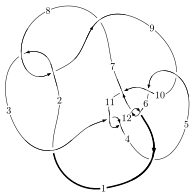
\includegraphics[width=112pt]{../../../GIT/diagram.site/Diagrams/png/1599_12a_0798.png}\\
\ \ \ A knot diagram\footnotemark}&
\allowdisplaybreaks
\textbf{Linearized knot diagam} \\
\cline{2-2}
 &
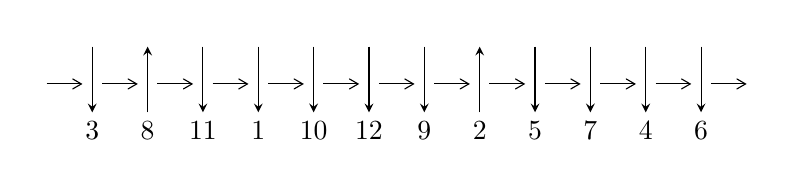
\begin{tikzpicture}[x=20pt, y=17pt]
	% nodes
	\node (C0) at (0, 0) {};
	\node (C1) at (1, 0) {};
	\node (C1U) at (1, +1) {};
	\node (C1D) at (1, -1) {3};

	\node (C2) at (2, 0) {};
	\node (C2U) at (2, +1) {};
	\node (C2D) at (2, -1) {8};

	\node (C3) at (3, 0) {};
	\node (C3U) at (3, +1) {};
	\node (C3D) at (3, -1) {11};

	\node (C4) at (4, 0) {};
	\node (C4U) at (4, +1) {};
	\node (C4D) at (4, -1) {1};

	\node (C5) at (5, 0) {};
	\node (C5U) at (5, +1) {};
	\node (C5D) at (5, -1) {10};

	\node (C6) at (6, 0) {};
	\node (C6U) at (6, +1) {};
	\node (C6D) at (6, -1) {12};

	\node (C7) at (7, 0) {};
	\node (C7U) at (7, +1) {};
	\node (C7D) at (7, -1) {9};

	\node (C8) at (8, 0) {};
	\node (C8U) at (8, +1) {};
	\node (C8D) at (8, -1) {2};

	\node (C9) at (9, 0) {};
	\node (C9U) at (9, +1) {};
	\node (C9D) at (9, -1) {5};

	\node (C10) at (10, 0) {};
	\node (C10U) at (10, +1) {};
	\node (C10D) at (10, -1) {7};

	\node (C11) at (11, 0) {};
	\node (C11U) at (11, +1) {};
	\node (C11D) at (11, -1) {4};

	\node (C12) at (12, 0) {};
	\node (C12U) at (12, +1) {};
	\node (C12D) at (12, -1) {6};
	\node (C13) at (13, 0) {};

	% arrows
	\draw[->,>={angle 60}]
	(C0) edge (C1) (C1) edge (C2) (C2) edge (C3) (C3) edge (C4) (C4) edge (C5) (C5) edge (C6) (C6) edge (C7) (C7) edge (C8) (C8) edge (C9) (C9) edge (C10) (C10) edge (C11) (C11) edge (C12) (C12) edge (C13) ;	\draw[->,>=stealth]
	(C1U) edge (C1D) (C2D) edge (C2U) (C3U) edge (C3D) (C4U) edge (C4D) (C5U) edge (C5D) (C6U) edge (C6D) (C7U) edge (C7D) (C8D) edge (C8U) (C9U) edge (C9D) (C10U) edge (C10D) (C11U) edge (C11D) (C12U) edge (C12D) ;
	\end{tikzpicture} \\
\hhline{~~} \\& 
\textbf{Solving Sequence} \\ \cline{2-2} 
 &
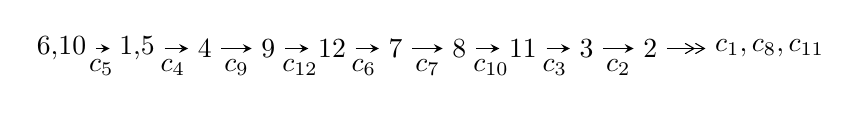
\begin{tikzpicture}[x=23pt, y=7pt]
	% node
	\node (A0) at (-1/8, 0) {6,10};
	\node (A1) at (17/16, 0) {1,5};
	\node (A2) at (17/8, 0) {4};
	\node (A3) at (25/8, 0) {9};
	\node (A4) at (33/8, 0) {12};
	\node (A5) at (41/8, 0) {7};
	\node (A6) at (49/8, 0) {8};
	\node (A7) at (57/8, 0) {11};
	\node (A8) at (65/8, 0) {3};
	\node (A9) at (73/8, 0) {2};
	\node (C1) at (1/2, -1) {$c_{5}$};
	\node (C2) at (13/8, -1) {$c_{4}$};
	\node (C3) at (21/8, -1) {$c_{9}$};
	\node (C4) at (29/8, -1) {$c_{12}$};
	\node (C5) at (37/8, -1) {$c_{6}$};
	\node (C6) at (45/8, -1) {$c_{7}$};
	\node (C7) at (53/8, -1) {$c_{10}$};
	\node (C8) at (61/8, -1) {$c_{3}$};
	\node (C9) at (69/8, -1) {$c_{2}$};
	\node (A10) at (11, 0) {$c_{1},c_{8},c_{11}$};

	% edge
	\draw[->,>=stealth]	
	(A0) edge (A1) (A1) edge (A2) (A2) edge (A3) (A3) edge (A4) (A4) edge (A5) (A5) edge (A6) (A6) edge (A7) (A7) edge (A8) (A8) edge (A9) ;
	\draw[->>,>={angle 60}]	
	(A9) edge (A10);
\end{tikzpicture} \\ 

\end{tabular} \\

\footnotetext{
The image of knot diagram is generated by the software ``\textbf{Draw programme}" developed by Andrew Bartholomew(\url{http://www.layer8.co.uk/maths/draw/index.htm\#Running-draw}), where we modified some parts for our purpose(\url{https://github.com/CATsTAILs/LinksPainter}).
}\phantom \\ \newline 
\centering \textbf{Ideals for irreducible components\footnotemark of $X_{\text{par}}$} 
 
\begin{align*}
I^u_{1}&=\langle 
2.00309\times10^{43} u^{48}-3.21474\times10^{41} u^{47}+\cdots+9.90975\times10^{43} b-9.19958\times10^{43},\\
\phantom{I^u_{1}}&\phantom{= \langle  }-3.05614\times10^{43} u^{48}-3.56503\times10^{41} u^{47}+\cdots+4.95488\times10^{43} a+3.30827\times10^{44},\;u^{49}+u^{48}+\cdots+8 u+1\rangle \\
I^u_{2}&=\langle 
2.20369\times10^{113} u^{69}+5.25148\times10^{112} u^{68}+\cdots+2.19562\times10^{115} b+2.18119\times10^{115},\\
\phantom{I^u_{2}}&\phantom{= \langle  }5.47739\times10^{116} u^{69}+3.09471\times10^{115} u^{68}+\cdots+1.16368\times10^{117} a+1.96706\times10^{118},\\
\phantom{I^u_{2}}&\phantom{= \langle  }u^{70}+u^{69}+\cdots+434 u+53\rangle \\
I^u_{3}&=\langle 
300 a^3+95 a^2+2260 b+654 a-1651,\;25 a^4-40 a^3-98 a^2+64 a+197,\;u+1\rangle \\
I^u_{4}&=\langle 
b+u,\;8 a^3+12 a^2 u-4 a^2-4 a u-2 a+u,\;u^2+1\rangle \\
I^u_{5}&=\langle 
- a^2+8 b+2 a+3,\;a^3+3 a^2+3 a+1,\;u-1\rangle \\
\\
\end{align*}
\raggedright * 5 irreducible components of $\dim_{\mathbb{C}}=0$, with total 132 representations.\\
\footnotetext{All coefficients of polynomials are rational numbers. But the coefficients are sometimes approximated in decimal forms when there is not enough margin.}
\newpage
\renewcommand{\arraystretch}{1}
\centering \section*{I. $I^u_{1}= \langle 2.00\times10^{43} u^{48}-3.21\times10^{41} u^{47}+\cdots+9.91\times10^{43} b-9.20\times10^{43},\;-3.06\times10^{43} u^{48}-3.57\times10^{41} u^{47}+\cdots+4.95\times10^{43} a+3.31\times10^{44},\;u^{49}+u^{48}+\cdots+8 u+1 \rangle$}
\flushleft \textbf{(i) Arc colorings}\\
\begin{tabular}{m{7pt} m{180pt} m{7pt} m{180pt} }
\flushright $a_{6}=$&$\begin{pmatrix}1\\0\end{pmatrix}$ \\
\flushright $a_{10}=$&$\begin{pmatrix}0\\u\end{pmatrix}$ \\
\flushright $a_{1}=$&$\begin{pmatrix}0.616794 u^{48}+0.00719500 u^{47}+\cdots-24.9481 u-6.67680\\-0.202134 u^{48}+0.00324402 u^{47}+\cdots+4.56122 u+0.928336\end{pmatrix}$ \\
\flushright $a_{5}=$&$\begin{pmatrix}1\\- u^2\end{pmatrix}$ \\
\flushright $a_{4}=$&$\begin{pmatrix}2.44394 u^{48}+2.29985 u^{47}+\cdots+67.1776 u+6.08652\\-0.404222 u^{48}-0.323237 u^{47}+\cdots-9.06575 u-0.414661\end{pmatrix}$ \\
\flushright $a_{9}=$&$\begin{pmatrix}u\\- u^3+u\end{pmatrix}$ \\
\flushright $a_{12}=$&$\begin{pmatrix}0.414661 u^{48}+0.0104390 u^{47}+\cdots-20.3869 u-5.74847\\-0.202134 u^{48}+0.00324402 u^{47}+\cdots+4.56122 u+0.928336\end{pmatrix}$ \\
\flushright $a_{7}=$&$\begin{pmatrix}-1.53794 u^{48}-1.54132 u^{47}+\cdots-47.9985 u-3.48227\\0.344085 u^{48}+0.255951 u^{47}+\cdots+7.86170 u+0.499407\end{pmatrix}$ \\
\flushright $a_{8}=$&$\begin{pmatrix}-1.51259 u^{48}-1.48491 u^{47}+\cdots-47.1606 u-3.63014\\0.434697 u^{48}+0.337745 u^{47}+\cdots+8.97345 u+0.382603\end{pmatrix}$ \\
\flushright $a_{11}=$&$\begin{pmatrix}0.270574 u^{48}-0.255160 u^{47}+\cdots-33.8519 u-8.19241\\-0.121149 u^{48}+0.0602775 u^{47}+\cdots+7.38033 u+1.33256\end{pmatrix}$ \\
\flushright $a_{3}=$&$\begin{pmatrix}2.96967 u^{48}+2.72241 u^{47}+\cdots+77.5346 u+6.35709\\-0.585648 u^{48}-0.423585 u^{47}+\cdots-11.3675 u-0.535810\end{pmatrix}$ \\
\flushright $a_{2}=$&$\begin{pmatrix}0.858872 u^{48}+1.20916 u^{47}+\cdots+51.2976 u+8.24260\\-0.477090 u^{48}-0.426611 u^{47}+\cdots-15.0209 u-2.17841\end{pmatrix}$\\&\end{tabular}
\flushleft \textbf{(ii) Obstruction class $= -1$}\\~\\
\flushleft \textbf{(iii) Cusp Shapes $= -3.15453 u^{48}-2.18463 u^{47}+\cdots-60.6939 u-13.0765$}\\~\\
\newpage\renewcommand{\arraystretch}{1}
\flushleft \textbf{(iv) u-Polynomials at the component}\newline \\
\begin{tabular}{m{50pt}|m{274pt}}
Crossings & \hspace{64pt}u-Polynomials at each crossing \\
\hline $$\begin{aligned}c_{1},c_{7}\end{aligned}$$&$\begin{aligned}
&u^{49}+17 u^{48}+\cdots-236 u-100
\end{aligned}$\\
\hline $$\begin{aligned}c_{2},c_{8}\end{aligned}$$&$\begin{aligned}
&u^{49}-3 u^{48}+\cdots+22 u+10
\end{aligned}$\\
\hline $$\begin{aligned}c_{3},c_{5},c_{9}\\c_{11}\end{aligned}$$&$\begin{aligned}
&u^{49}+u^{48}+\cdots+8 u+1
\end{aligned}$\\
\hline $$\begin{aligned}c_{4},c_{10}\end{aligned}$$&$\begin{aligned}
&64(64 u^{49}-128 u^{48}+\cdots+20 u+1)
\end{aligned}$\\
\hline $$\begin{aligned}c_{6},c_{12}\end{aligned}$$&$\begin{aligned}
&u^{49}+3 u^{48}+\cdots+186 u+50
\end{aligned}$\\
\hline
\end{tabular}\\~\\
\newpage\renewcommand{\arraystretch}{1}
\flushleft \textbf{(v) Riley Polynomials at the component}\newline \\
\begin{tabular}{m{50pt}|m{274pt}}
Crossings & \hspace{64pt}Riley Polynomials at each crossing \\
\hline $$\begin{aligned}c_{1},c_{7}\end{aligned}$$&$\begin{aligned}
&y^{49}+33 y^{48}+\cdots-115504 y-10000
\end{aligned}$\\
\hline $$\begin{aligned}c_{2},c_{8}\end{aligned}$$&$\begin{aligned}
&y^{49}+17 y^{48}+\cdots-236 y-100
\end{aligned}$\\
\hline $$\begin{aligned}c_{3},c_{5},c_{9}\\c_{11}\end{aligned}$$&$\begin{aligned}
&y^{49}-15 y^{48}+\cdots-16 y-1
\end{aligned}$\\
\hline $$\begin{aligned}c_{4},c_{10}\end{aligned}$$&$\begin{aligned}
&4096(4096 y^{49}+73728 y^{48}+\cdots-62 y-1)
\end{aligned}$\\
\hline $$\begin{aligned}c_{6},c_{12}\end{aligned}$$&$\begin{aligned}
&y^{49}+21 y^{48}+\cdots-112004 y-2500
\end{aligned}$\\
\hline
\end{tabular}\\~\\
\newpage\flushleft \textbf{(vi) Complex Volumes and Cusp Shapes}
$$\begin{array}{c|c|c}  
\text{Solutions to }I^u_{1}& \I (\text{vol} + \sqrt{-1}CS) & \text{Cusp shape}\\
 \hline 
\begin{aligned}
u &= \phantom{-}0.981538 + 0.257391 I \\
a &= \phantom{-}1.55206 - 0.93078 I \\
b &= -1.23894 + 0.72248 I\end{aligned}
 & -5.77516 + 2.35068 I & -11.35180 + 4.63129 I \\ \hline\begin{aligned}
u &= \phantom{-}0.981538 - 0.257391 I \\
a &= \phantom{-}1.55206 + 0.93078 I \\
b &= -1.23894 - 0.72248 I\end{aligned}
 & -5.77516 - 2.35068 I & -11.35180 - 4.63129 I \\ \hline\begin{aligned}
u &= -0.810441 + 0.532063 I \\
a &= \phantom{-}2.11896 - 0.39965 I \\
b &= -0.643779 + 0.920170 I\end{aligned}
 & \phantom{-}5.03502 + 0.73563 I & -5.79688 - 4.57205 I \\ \hline\begin{aligned}
u &= -0.810441 - 0.532063 I \\
a &= \phantom{-}2.11896 + 0.39965 I \\
b &= -0.643779 - 0.920170 I\end{aligned}
 & \phantom{-}5.03502 - 0.73563 I & -5.79688 + 4.57205 I \\ \hline\begin{aligned}
u &= \phantom{-}0.877698 + 0.561491 I \\
a &= -2.08820 - 0.30060 I \\
b &= \phantom{-}0.653043 + 0.991957 I\end{aligned}
 & \phantom{-}5.31366 - 7.02170 I & -5.51690 + 9.17495 I \\ \hline\begin{aligned}
u &= \phantom{-}0.877698 - 0.561491 I \\
a &= -2.08820 + 0.30060 I \\
b &= \phantom{-}0.653043 - 0.991957 I\end{aligned}
 & \phantom{-}5.31366 + 7.02170 I & -5.51690 - 9.17495 I \\ \hline\begin{aligned}
u &= -0.995699 + 0.372749 I \\
a &= -1.36330 - 0.86812 I \\
b &= \phantom{-}1.104890 + 0.550579 I\end{aligned}
 & -3.06110 + 2.74516 I & -8.49807 - 6.15151 I \\ \hline\begin{aligned}
u &= -0.995699 - 0.372749 I \\
a &= -1.36330 + 0.86812 I \\
b &= \phantom{-}1.104890 - 0.550579 I\end{aligned}
 & -3.06110 - 2.74516 I & -8.49807 + 6.15151 I \\ \hline\begin{aligned}
u &= \phantom{-}0.875340 + 0.605659 I \\
a &= \phantom{-}0.219349 + 0.234083 I \\
b &= \phantom{-}0.214791 - 1.396630 I\end{aligned}
 & \phantom{-}5.30349 - 2.15840 I & -3.93083 + 3.29725 I \\ \hline\begin{aligned}
u &= \phantom{-}0.875340 - 0.605659 I \\
a &= \phantom{-}0.219349 - 0.234083 I \\
b &= \phantom{-}0.214791 + 1.396630 I\end{aligned}
 & \phantom{-}5.30349 + 2.15840 I & -3.93083 - 3.29725 I\\
 \hline 
 \end{array}$$\newpage$$\begin{array}{c|c|c}  
\text{Solutions to }I^u_{1}& \I (\text{vol} + \sqrt{-1}CS) & \text{Cusp shape}\\
 \hline 
\begin{aligned}
u &= -0.952373 + 0.520378 I \\
a &= -0.168176 + 0.392073 I \\
b &= -0.22875 - 1.47692 I\end{aligned}
 & \phantom{-}4.08293 + 7.70387 I & -6.80678 - 8.64886 I \\ \hline\begin{aligned}
u &= -0.952373 - 0.520378 I \\
a &= -0.168176 - 0.392073 I \\
b &= -0.22875 + 1.47692 I\end{aligned}
 & \phantom{-}4.08293 - 7.70387 I & -6.80678 + 8.64886 I \\ \hline\begin{aligned}
u &= \phantom{-}0.452697 + 0.787769 I \\
a &= \phantom{-}0.288931 - 0.311418 I \\
b &= \phantom{-}0.127804 - 1.164260 I\end{aligned}
 & \phantom{-}3.71295 - 0.68830 I & \phantom{-}0.52323 + 2.74701 I \\ \hline\begin{aligned}
u &= \phantom{-}0.452697 - 0.787769 I \\
a &= \phantom{-}0.288931 + 0.311418 I \\
b &= \phantom{-}0.127804 + 1.164260 I\end{aligned}
 & \phantom{-}3.71295 + 0.68830 I & \phantom{-}0.52323 - 2.74701 I \\ \hline\begin{aligned}
u &= \phantom{-}0.817518 + 0.099039 I \\
a &= -2.07999 - 0.26336 I \\
b &= \phantom{-}1.288930 + 0.381664 I\end{aligned}
 & -4.95390 - 4.13277 I & -5.04587 + 8.33177 I \\ \hline\begin{aligned}
u &= \phantom{-}0.817518 - 0.099039 I \\
a &= -2.07999 + 0.26336 I \\
b &= \phantom{-}1.288930 - 0.381664 I\end{aligned}
 & -4.95390 + 4.13277 I & -5.04587 - 8.33177 I \\ \hline\begin{aligned}
u &= \phantom{-}1.147530 + 0.376229 I \\
a &= \phantom{-}1.35388 - 0.64687 I \\
b &= -1.218000 + 0.378064 I\end{aligned}
 & -8.08094 - 5.83164 I & -15.5949 + 6.7506 I \\ \hline\begin{aligned}
u &= \phantom{-}1.147530 - 0.376229 I \\
a &= \phantom{-}1.35388 + 0.64687 I \\
b &= -1.218000 - 0.378064 I\end{aligned}
 & -8.08094 + 5.83164 I & -15.5949 - 6.7506 I \\ \hline\begin{aligned}
u &= -1.137970 + 0.439927 I \\
a &= \phantom{-}1.72337 - 0.29059 I \\
b &= -0.79502 + 1.21714 I\end{aligned}
 & -3.88494 + 4.95670 I & -12.24760 - 4.43222 I \\ \hline\begin{aligned}
u &= -1.137970 - 0.439927 I \\
a &= \phantom{-}1.72337 + 0.29059 I \\
b &= -0.79502 - 1.21714 I\end{aligned}
 & -3.88494 - 4.95670 I & -12.24760 + 4.43222 I\\
 \hline 
 \end{array}$$\newpage$$\begin{array}{c|c|c}  
\text{Solutions to }I^u_{1}& \I (\text{vol} + \sqrt{-1}CS) & \text{Cusp shape}\\
 \hline 
\begin{aligned}
u &= -0.688687 + 0.308958 I \\
a &= -0.878871 + 0.471910 I \\
b &= \phantom{-}0.07117 - 1.41606 I\end{aligned}
 & -0.16229 + 1.40976 I & -9.53355 - 4.57288 I \\ \hline\begin{aligned}
u &= -0.688687 - 0.308958 I \\
a &= -0.878871 - 0.471910 I \\
b &= \phantom{-}0.07117 + 1.41606 I\end{aligned}
 & -0.16229 - 1.40976 I & -9.53355 + 4.57288 I \\ \hline\begin{aligned}
u &= -0.286451 + 1.239410 I \\
a &= \phantom{-}0.020365 - 0.390591 I \\
b &= -0.214987 - 0.936488 I\end{aligned}
 & \phantom{-}1.83503 - 0.92197 I & -13.0094 + 8.1328 I \\ \hline\begin{aligned}
u &= -0.286451 - 1.239410 I \\
a &= \phantom{-}0.020365 + 0.390591 I \\
b &= -0.214987 + 0.936488 I\end{aligned}
 & \phantom{-}1.83503 + 0.92197 I & -13.0094 - 8.1328 I \\ \hline\begin{aligned}
u &= \phantom{-}1.156850 + 0.550225 I \\
a &= -1.74873 - 0.14409 I \\
b &= \phantom{-}0.706757 + 1.215220 I\end{aligned}
 & -0.79278 - 9.29438 I & -8.00000 + 7.50073 I \\ \hline\begin{aligned}
u &= \phantom{-}1.156850 - 0.550225 I \\
a &= -1.74873 + 0.14409 I \\
b &= \phantom{-}0.706757 - 1.215220 I\end{aligned}
 & -0.79278 + 9.29438 I & -8.00000 - 7.50073 I \\ \hline\begin{aligned}
u &= -1.163070 + 0.539405 I \\
a &= -1.160470 - 0.653820 I \\
b &= \phantom{-}1.087680 + 0.283705 I\end{aligned}
 & -0.80094 + 6.65775 I & -8.00000 + 0. I\phantom{ +0.000000I} \\ \hline\begin{aligned}
u &= -1.163070 - 0.539405 I \\
a &= -1.160470 + 0.653820 I \\
b &= \phantom{-}1.087680 - 0.283705 I\end{aligned}
 & -0.80094 - 6.65775 I & -8.00000 + 0. I\phantom{ +0.000000I} \\ \hline\begin{aligned}
u &= -0.079925 + 0.692755 I \\
a &= -0.057126 - 1.297370 I \\
b &= \phantom{-}0.053644 + 0.267090 I\end{aligned}
 & \phantom{-}4.56105 + 2.90065 I & -5.11259 - 3.32387 I \\ \hline\begin{aligned}
u &= -0.079925 - 0.692755 I \\
a &= -0.057126 + 1.297370 I \\
b &= \phantom{-}0.053644 - 0.267090 I\end{aligned}
 & \phantom{-}4.56105 - 2.90065 I & -5.11259 + 3.32387 I\\
 \hline 
 \end{array}$$\newpage$$\begin{array}{c|c|c}  
\text{Solutions to }I^u_{1}& \I (\text{vol} + \sqrt{-1}CS) & \text{Cusp shape}\\
 \hline 
\begin{aligned}
u &= -0.021549 + 1.328260 I \\
a &= \phantom{-}0.023794 - 0.515824 I \\
b &= -0.058851 - 0.693519 I\end{aligned}
 & \phantom{-}5.08062 + 2.68757 I & -8.00000 + 0. I\phantom{ +0.000000I} \\ \hline\begin{aligned}
u &= -0.021549 - 1.328260 I \\
a &= \phantom{-}0.023794 + 0.515824 I \\
b &= -0.058851 + 0.693519 I\end{aligned}
 & \phantom{-}5.08062 - 2.68757 I & -8.00000 + 0. I\phantom{ +0.000000I} \\ \hline\begin{aligned}
u &= -0.671080\phantom{ +0.000000I} \\
a &= \phantom{-}1.79535\phantom{ +0.000000I} \\
b &= -0.940047\phantom{ +0.000000I}\end{aligned}
 & -1.58789\phantom{ +0.000000I} & -4.29000\phantom{ +0.000000I} \\ \hline\begin{aligned}
u &= \phantom{-}1.220900 + 0.538472 I \\
a &= \phantom{-}1.155260 - 0.596939 I \\
b &= -1.115300 + 0.247129 I\end{aligned}
 & -2.05345 - 12.68030 I & \phantom{-0.000000 } 0 \\ \hline\begin{aligned}
u &= \phantom{-}1.220900 - 0.538472 I \\
a &= \phantom{-}1.155260 + 0.596939 I \\
b &= -1.115300 - 0.247129 I\end{aligned}
 & -2.05345 + 12.68030 I & \phantom{-0.000000 } 0 \\ \hline\begin{aligned}
u &= \phantom{-}0.627660 + 1.221110 I \\
a &= -0.031390 - 0.235628 I \\
b &= \phantom{-}0.331694 - 1.079920 I\end{aligned}
 & \phantom{-}7.31454 - 0.58694 I & \phantom{-0.000000 } 0 \\ \hline\begin{aligned}
u &= \phantom{-}0.627660 - 1.221110 I \\
a &= -0.031390 + 0.235628 I \\
b &= \phantom{-}0.331694 + 1.079920 I\end{aligned}
 & \phantom{-}7.31454 + 0.58694 I & \phantom{-0.000000 } 0 \\ \hline\begin{aligned}
u &= -1.260280 + 0.553994 I \\
a &= \phantom{-}1.62317 - 0.09420 I \\
b &= -0.69242 + 1.27875 I\end{aligned}
 & -5.13578 + 12.53380 I & \phantom{-0.000000 } 0 \\ \hline\begin{aligned}
u &= -1.260280 - 0.553994 I \\
a &= \phantom{-}1.62317 + 0.09420 I \\
b &= -0.69242 - 1.27875 I\end{aligned}
 & -5.13578 - 12.53380 I & \phantom{-0.000000 } 0 \\ \hline\begin{aligned}
u &= -0.58514 + 1.29446 I \\
a &= \phantom{-}0.057217 - 0.263592 I \\
b &= -0.345871 - 1.041880 I\end{aligned}
 & \phantom{-}6.79396 - 5.08385 I & \phantom{-0.000000 } 0\\
 \hline 
 \end{array}$$\newpage$$\begin{array}{c|c|c}  
\text{Solutions to }I^u_{1}& \I (\text{vol} + \sqrt{-1}CS) & \text{Cusp shape}\\
 \hline 
\begin{aligned}
u &= -0.58514 - 1.29446 I \\
a &= \phantom{-}0.057217 + 0.263592 I \\
b &= -0.345871 + 1.041880 I\end{aligned}
 & \phantom{-}6.79396 + 5.08385 I & \phantom{-0.000000 } 0 \\ \hline\begin{aligned}
u &= \phantom{-}1.25870 + 0.66450 I \\
a &= -1.66771 + 0.03866 I \\
b &= \phantom{-}0.63511 + 1.26857 I\end{aligned}
 & \phantom{-}2.30602 - 12.80540 I & \phantom{-0.000000 } 0 \\ \hline\begin{aligned}
u &= \phantom{-}1.25870 - 0.66450 I \\
a &= -1.66771 - 0.03866 I \\
b &= \phantom{-}0.63511 - 1.26857 I\end{aligned}
 & \phantom{-}2.30602 + 12.80540 I & \phantom{-0.000000 } 0 \\ \hline\begin{aligned}
u &= -1.29293 + 0.66685 I \\
a &= \phantom{-}1.62720 + 0.05274 I \\
b &= -0.63273 + 1.28478 I\end{aligned}
 & \phantom{-}1.2109 + 18.8792 I & \phantom{-0.000000 } 0 \\ \hline\begin{aligned}
u &= -1.29293 - 0.66685 I \\
a &= \phantom{-}1.62720 - 0.05274 I \\
b &= -0.63273 - 1.28478 I\end{aligned}
 & \phantom{-}1.2109 - 18.8792 I & \phantom{-0.000000 } 0 \\ \hline\begin{aligned}
u &= -0.208725 + 0.263076 I \\
a &= \phantom{-}0.636904 - 0.809965 I \\
b &= -0.176417 + 0.283511 I\end{aligned}
 & -0.386214 + 0.820546 I & -8.61529 - 8.26097 I \\ \hline\begin{aligned}
u &= -0.208725 - 0.263076 I \\
a &= \phantom{-}0.636904 + 0.809965 I \\
b &= -0.176417 - 0.283511 I\end{aligned}
 & -0.386214 - 0.820546 I & -8.61529 + 8.26097 I \\ \hline\begin{aligned}
u &= -0.097656 + 0.221062 I \\
a &= -1.55418 - 4.92473 I \\
b &= \phantom{-}0.055569 + 0.876388 I\end{aligned}
 & \phantom{-}4.71535 + 2.88833 I & -6.61461 - 3.16484 I \\ \hline\begin{aligned}
u &= -0.097656 - 0.221062 I \\
a &= -1.55418 + 4.92473 I \\
b &= \phantom{-}0.055569 - 0.876388 I\end{aligned}
 & \phantom{-}4.71535 - 2.88833 I & -6.61461 + 3.16484 I\\
 \hline 
 \end{array}$$\newpage\newpage\renewcommand{\arraystretch}{1}
\centering \section*{II. $I^u_{2}= \langle 2.20\times10^{113} u^{69}+5.25\times10^{112} u^{68}+\cdots+2.20\times10^{115} b+2.18\times10^{115},\;5.48\times10^{116} u^{69}+3.09\times10^{115} u^{68}+\cdots+1.16\times10^{117} a+1.97\times10^{118},\;u^{70}+u^{69}+\cdots+434 u+53 \rangle$}
\flushleft \textbf{(i) Arc colorings}\\
\begin{tabular}{m{7pt} m{180pt} m{7pt} m{180pt} }
\flushright $a_{6}=$&$\begin{pmatrix}1\\0\end{pmatrix}$ \\
\flushright $a_{10}=$&$\begin{pmatrix}0\\u\end{pmatrix}$ \\
\flushright $a_{1}=$&$\begin{pmatrix}-0.470697 u^{69}-0.0265942 u^{68}+\cdots-149.260 u-16.9039\\-0.0100368 u^{69}-0.00239180 u^{68}+\cdots-2.54768 u-0.993431\end{pmatrix}$ \\
\flushright $a_{5}=$&$\begin{pmatrix}1\\- u^2\end{pmatrix}$ \\
\flushright $a_{4}=$&$\begin{pmatrix}-6.01017 u^{69}+0.310008 u^{68}+\cdots-2255.61 u-308.627\\-0.226244 u^{69}+0.0311423 u^{68}+\cdots-77.8654 u-11.1406\end{pmatrix}$ \\
\flushright $a_{9}=$&$\begin{pmatrix}u\\- u^3+u\end{pmatrix}$ \\
\flushright $a_{12}=$&$\begin{pmatrix}-0.480734 u^{69}-0.0289860 u^{68}+\cdots-151.807 u-17.8973\\-0.0100368 u^{69}-0.00239180 u^{68}+\cdots-2.54768 u-0.993431\end{pmatrix}$ \\
\flushright $a_{7}=$&$\begin{pmatrix}0.155671 u^{69}-0.0389813 u^{68}+\cdots+43.7618 u+4.64741\\-0.0580571 u^{69}-0.00135076 u^{68}+\cdots-19.8965 u-2.18136\end{pmatrix}$ \\
\flushright $a_{8}=$&$\begin{pmatrix}0.143997 u^{69}-0.0275353 u^{68}+\cdots+38.2166 u+3.85369\\-0.0460225 u^{69}+0.0000400031 u^{68}+\cdots-16.0263 u-1.74972\end{pmatrix}$ \\
\flushright $a_{11}=$&$\begin{pmatrix}-6.43551 u^{69}+0.0646646 u^{68}+\cdots-2338.34 u-323.669\\-0.222739 u^{69}+0.0292459 u^{68}+\cdots-71.9426 u-10.0199\end{pmatrix}$ \\
\flushright $a_{3}=$&$\begin{pmatrix}0.120256 u^{69}-0.0236167 u^{68}+\cdots+41.4888 u+9.39135\\-0.0209187 u^{69}+0.000811014 u^{68}+\cdots-9.03896 u-1.96341\end{pmatrix}$ \\
\flushright $a_{2}=$&$\begin{pmatrix}0.363436 u^{69}+0.0187985 u^{68}+\cdots+118.612 u+19.4997\\0.00913425 u^{69}-0.000942294 u^{68}+\cdots+1.20552 u-0.169703\end{pmatrix}$\\&\end{tabular}
\flushleft \textbf{(ii) Obstruction class $= -1$}\\~\\
\flushleft \textbf{(iii) Cusp Shapes $= 0.0239601 u^{69}-0.00841492 u^{68}+\cdots+18.6490 u-3.90520$}\\~\\
\newpage\renewcommand{\arraystretch}{1}
\flushleft \textbf{(iv) u-Polynomials at the component}\newline \\
\begin{tabular}{m{50pt}|m{274pt}}
Crossings & \hspace{64pt}u-Polynomials at each crossing \\
\hline $$\begin{aligned}c_{1},c_{7}\end{aligned}$$&$\begin{aligned}
&(u^{35}+11 u^{34}+\cdots-2 u-1)^{2}
\end{aligned}$\\
\hline $$\begin{aligned}c_{2},c_{8}\end{aligned}$$&$\begin{aligned}
&(u^{35}+u^{34}+\cdots+2 u+1)^{2}
\end{aligned}$\\
\hline $$\begin{aligned}c_{3},c_{5},c_{9}\\c_{11}\end{aligned}$$&$\begin{aligned}
&u^{70}+u^{69}+\cdots+434 u+53
\end{aligned}$\\
\hline $$\begin{aligned}c_{4},c_{10}\end{aligned}$$&$\begin{aligned}
&u^{70}+19 u^{69}+\cdots+60600 u-5375
\end{aligned}$\\
\hline $$\begin{aligned}c_{6},c_{12}\end{aligned}$$&$\begin{aligned}
&(u^{35}- u^{34}+\cdots-2 u+1)^{2}
\end{aligned}$\\
\hline
\end{tabular}\\~\\
\newpage\renewcommand{\arraystretch}{1}
\flushleft \textbf{(v) Riley Polynomials at the component}\newline \\
\begin{tabular}{m{50pt}|m{274pt}}
Crossings & \hspace{64pt}Riley Polynomials at each crossing \\
\hline $$\begin{aligned}c_{1},c_{7}\end{aligned}$$&$\begin{aligned}
&(y^{35}+27 y^{34}+\cdots-22 y-1)^{2}
\end{aligned}$\\
\hline $$\begin{aligned}c_{2},c_{8}\end{aligned}$$&$\begin{aligned}
&(y^{35}+11 y^{34}+\cdots-2 y-1)^{2}
\end{aligned}$\\
\hline $$\begin{aligned}c_{3},c_{5},c_{9}\\c_{11}\end{aligned}$$&$\begin{aligned}
&y^{70}-41 y^{69}+\cdots-86596 y+2809
\end{aligned}$\\
\hline $$\begin{aligned}c_{4},c_{10}\end{aligned}$$&$\begin{aligned}
&y^{70}-21 y^{69}+\cdots-1096015000 y+28890625
\end{aligned}$\\
\hline $$\begin{aligned}c_{6},c_{12}\end{aligned}$$&$\begin{aligned}
&(y^{35}+19 y^{34}+\cdots-2 y-1)^{2}
\end{aligned}$\\
\hline
\end{tabular}\\~\\
\newpage\flushleft \textbf{(vi) Complex Volumes and Cusp Shapes}
$$\begin{array}{c|c|c}  
\text{Solutions to }I^u_{2}& \I (\text{vol} + \sqrt{-1}CS) & \text{Cusp shape}\\
 \hline 
\begin{aligned}
u &= -0.119514 + 1.003680 I \\
a &= -0.124946 + 0.339745 I \\
b &= \phantom{-}0.491471 + 1.162520 I\end{aligned}
 & -1.63653 - 7.02473 I & -10.39842 + 6.93954 I \\ \hline\begin{aligned}
u &= -0.119514 - 1.003680 I \\
a &= -0.124946 - 0.339745 I \\
b &= \phantom{-}0.491471 - 1.162520 I\end{aligned}
 & -1.63653 + 7.02473 I & -10.39842 - 6.93954 I \\ \hline\begin{aligned}
u &= \phantom{-}0.967240 + 0.057432 I \\
a &= \phantom{-}2.54114 - 12.61520 I \\
b &= \phantom{-}0.030366 - 1.049680 I\end{aligned}
 & \phantom{-}1.36125 + 2.79178 I & -2.56555 - 3.12849 I \\ \hline\begin{aligned}
u &= \phantom{-}0.967240 - 0.057432 I \\
a &= \phantom{-}2.54114 + 12.61520 I \\
b &= \phantom{-}0.030366 + 1.049680 I\end{aligned}
 & \phantom{-}1.36125 - 2.79178 I & -2.56555 + 3.12849 I \\ \hline\begin{aligned}
u &= -1.037220 + 0.046542 I \\
a &= -11.49130 - 3.57082 I \\
b &= \phantom{-}0.030366 - 1.049680 I\end{aligned}
 & \phantom{-}1.36125 + 2.79178 I & -2.56555 - 3.12849 I \\ \hline\begin{aligned}
u &= -1.037220 - 0.046542 I \\
a &= -11.49130 + 3.57082 I \\
b &= \phantom{-}0.030366 + 1.049680 I\end{aligned}
 & \phantom{-}1.36125 - 2.79178 I & -2.56555 + 3.12849 I \\ \hline\begin{aligned}
u &= \phantom{-}0.992816 + 0.307203 I \\
a &= -1.86835 + 0.59825 I \\
b &= \phantom{-}0.274169 + 0.754223 I\end{aligned}
 & -2.90212 - 1.21814 I & -7.56786 + 5.43737 I \\ \hline\begin{aligned}
u &= \phantom{-}0.992816 - 0.307203 I \\
a &= -1.86835 - 0.59825 I \\
b &= \phantom{-}0.274169 - 0.754223 I\end{aligned}
 & -2.90212 + 1.21814 I & -7.56786 - 5.43737 I \\ \hline\begin{aligned}
u &= \phantom{-}0.812668 + 0.700215 I \\
a &= -0.796936 + 1.003470 I \\
b &= \phantom{-}0.475306 + 0.917107 I\end{aligned}
 & -1.67002 - 2.07827 I & -8.00000 + 3.40333 I \\ \hline\begin{aligned}
u &= \phantom{-}0.812668 - 0.700215 I \\
a &= -0.796936 - 1.003470 I \\
b &= \phantom{-}0.475306 - 0.917107 I\end{aligned}
 & -1.67002 + 2.07827 I & -8.00000 - 3.40333 I\\
 \hline 
 \end{array}$$\newpage$$\begin{array}{c|c|c}  
\text{Solutions to }I^u_{2}& \I (\text{vol} + \sqrt{-1}CS) & \text{Cusp shape}\\
 \hline 
\begin{aligned}
u &= -1.041410 + 0.270926 I \\
a &= -1.52455 + 0.29351 I \\
b &= \phantom{-}0.407102 - 1.144230 I\end{aligned}
 & -1.01725 + 1.14078 I & -8.93962 + 0.35223 I \\ \hline\begin{aligned}
u &= -1.041410 - 0.270926 I \\
a &= -1.52455 - 0.29351 I \\
b &= \phantom{-}0.407102 + 1.144230 I\end{aligned}
 & -1.01725 - 1.14078 I & -8.93962 - 0.35223 I \\ \hline\begin{aligned}
u &= \phantom{-}0.133172 + 0.888260 I \\
a &= -0.513616 + 0.654211 I \\
b &= \phantom{-}0.817305 + 0.125028 I\end{aligned}
 & \phantom{-}1.19431 + 7.52211 I & -8.37393 - 5.45189 I \\ \hline\begin{aligned}
u &= \phantom{-}0.133172 - 0.888260 I \\
a &= -0.513616 - 0.654211 I \\
b &= \phantom{-}0.817305 - 0.125028 I\end{aligned}
 & \phantom{-}1.19431 - 7.52211 I & -8.37393 + 5.45189 I \\ \hline\begin{aligned}
u &= -0.977207 + 0.510227 I \\
a &= \phantom{-}0.223970 - 0.121731 I \\
b &= \phantom{-}0.510838 + 0.446804 I\end{aligned}
 & -2.91461 - 1.90476 I & -11.61760 + 3.26312 I \\ \hline\begin{aligned}
u &= -0.977207 - 0.510227 I \\
a &= \phantom{-}0.223970 + 0.121731 I \\
b &= \phantom{-}0.510838 - 0.446804 I\end{aligned}
 & -2.91461 + 1.90476 I & -11.61760 - 3.26312 I \\ \hline\begin{aligned}
u &= -0.895460\phantom{ +0.000000I} \\
a &= \phantom{-}1.21237\phantom{ +0.000000I} \\
b &= -0.714433\phantom{ +0.000000I}\end{aligned}
 & -1.48735\phantom{ +0.000000I} & -6.22320\phantom{ +0.000000I} \\ \hline\begin{aligned}
u &= -0.744917 + 0.469702 I \\
a &= -0.771318 - 0.328880 I \\
b &= \phantom{-}0.386425 + 1.221160 I\end{aligned}
 & \phantom{-}5.25248 + 3.42594 I & -3.89028 - 2.22817 I \\ \hline\begin{aligned}
u &= -0.744917 - 0.469702 I \\
a &= -0.771318 + 0.328880 I \\
b &= \phantom{-}0.386425 - 1.221160 I\end{aligned}
 & \phantom{-}5.25248 - 3.42594 I & -3.89028 + 2.22817 I \\ \hline\begin{aligned}
u &= \phantom{-}0.672202 + 0.568802 I \\
a &= \phantom{-}0.588099 - 0.277287 I \\
b &= -0.402291 + 1.220240 I\end{aligned}
 & \phantom{-}5.91946 + 2.50696 I & -2.73890 - 2.94934 I\\
 \hline 
 \end{array}$$\newpage$$\begin{array}{c|c|c}  
\text{Solutions to }I^u_{2}& \I (\text{vol} + \sqrt{-1}CS) & \text{Cusp shape}\\
 \hline 
\begin{aligned}
u &= \phantom{-}0.672202 - 0.568802 I \\
a &= \phantom{-}0.588099 + 0.277287 I \\
b &= -0.402291 - 1.220240 I\end{aligned}
 & \phantom{-}5.91946 - 2.50696 I & -2.73890 + 2.94934 I \\ \hline\begin{aligned}
u &= \phantom{-}0.657413 + 0.573036 I \\
a &= \phantom{-}1.95056 - 0.17929 I \\
b &= -0.402291 - 1.220240 I\end{aligned}
 & \phantom{-}5.91946 - 2.50696 I & -2.73890 + 2.94934 I \\ \hline\begin{aligned}
u &= \phantom{-}0.657413 - 0.573036 I \\
a &= \phantom{-}1.95056 + 0.17929 I \\
b &= -0.402291 + 1.220240 I\end{aligned}
 & \phantom{-}5.91946 + 2.50696 I & -2.73890 - 2.94934 I \\ \hline\begin{aligned}
u &= \phantom{-}0.276214 + 0.810444 I \\
a &= \phantom{-}0.0549455 + 0.0810153 I \\
b &= -0.453184 + 1.179210 I\end{aligned}
 & \phantom{-}1.83551 + 4.24996 I & -3.13542 - 3.77353 I \\ \hline\begin{aligned}
u &= \phantom{-}0.276214 - 0.810444 I \\
a &= \phantom{-}0.0549455 - 0.0810153 I \\
b &= -0.453184 - 1.179210 I\end{aligned}
 & \phantom{-}1.83551 - 4.24996 I & -3.13542 + 3.77353 I \\ \hline\begin{aligned}
u &= -0.223135 + 0.814237 I \\
a &= \phantom{-}0.614394 + 0.692076 I \\
b &= -0.812555 + 0.099238 I\end{aligned}
 & \phantom{-}1.97019 - 1.67857 I & -6.82266 + 0.36674 I \\ \hline\begin{aligned}
u &= -0.223135 - 0.814237 I \\
a &= \phantom{-}0.614394 - 0.692076 I \\
b &= -0.812555 - 0.099238 I\end{aligned}
 & \phantom{-}1.97019 + 1.67857 I & -6.82266 - 0.36674 I \\ \hline\begin{aligned}
u &= \phantom{-}0.337448 + 1.122360 I \\
a &= \phantom{-}0.279152 + 0.257589 I \\
b &= -0.498606 + 1.204550 I\end{aligned}
 & \phantom{-}5.23403 + 6.46046 I & \phantom{-0.000000 } 0 \\ \hline\begin{aligned}
u &= \phantom{-}0.337448 - 1.122360 I \\
a &= \phantom{-}0.279152 - 0.257589 I \\
b &= -0.498606 - 1.204550 I\end{aligned}
 & \phantom{-}5.23403 - 6.46046 I & \phantom{-0.000000 } 0 \\ \hline\begin{aligned}
u &= -1.165920 + 0.188060 I \\
a &= \phantom{-}0.066157 - 1.277360 I \\
b &= \phantom{-}0.274169 + 0.754223 I\end{aligned}
 & -2.90212 - 1.21814 I & \phantom{-0.000000 } 0\\
 \hline 
 \end{array}$$\newpage$$\begin{array}{c|c|c}  
\text{Solutions to }I^u_{2}& \I (\text{vol} + \sqrt{-1}CS) & \text{Cusp shape}\\
 \hline 
\begin{aligned}
u &= -1.165920 - 0.188060 I \\
a &= \phantom{-}0.066157 + 1.277360 I \\
b &= \phantom{-}0.274169 - 0.754223 I\end{aligned}
 & -2.90212 + 1.21814 I & \phantom{-0.000000 } 0 \\ \hline\begin{aligned}
u &= \phantom{-}1.068030 + 0.544420 I \\
a &= \phantom{-}1.46092 + 0.01825 I \\
b &= -0.453184 - 1.179210 I\end{aligned}
 & \phantom{-}1.83551 - 4.24996 I & \phantom{-0.000000 } 0 \\ \hline\begin{aligned}
u &= \phantom{-}1.068030 - 0.544420 I \\
a &= \phantom{-}1.46092 - 0.01825 I \\
b &= -0.453184 + 1.179210 I\end{aligned}
 & \phantom{-}1.83551 + 4.24996 I & \phantom{-0.000000 } 0 \\ \hline\begin{aligned}
u &= -0.298459 + 1.176530 I \\
a &= -0.284974 + 0.293575 I \\
b &= \phantom{-}0.509525 + 1.201690 I\end{aligned}
 & \phantom{-}4.37931 - 12.37660 I & \phantom{-0.000000 } 0 \\ \hline\begin{aligned}
u &= -0.298459 - 1.176530 I \\
a &= -0.284974 - 0.293575 I \\
b &= \phantom{-}0.509525 - 1.201690 I\end{aligned}
 & \phantom{-}4.37931 + 12.37660 I & \phantom{-0.000000 } 0 \\ \hline\begin{aligned}
u &= -1.101900 + 0.519411 I \\
a &= \phantom{-}0.959687 + 0.178430 I \\
b &= -0.812555 - 0.099238 I\end{aligned}
 & \phantom{-}1.97019 + 1.67857 I & \phantom{-0.000000 } 0 \\ \hline\begin{aligned}
u &= -1.101900 - 0.519411 I \\
a &= \phantom{-}0.959687 - 0.178430 I \\
b &= -0.812555 + 0.099238 I\end{aligned}
 & \phantom{-}1.97019 - 1.67857 I & \phantom{-0.000000 } 0 \\ \hline\begin{aligned}
u &= \phantom{-}1.205300 + 0.207889 I \\
a &= -1.031590 + 0.049162 I \\
b &= \phantom{-}0.703066 - 0.147767 I\end{aligned}
 & -4.55305 - 2.51214 I & \phantom{-0.000000 } 0 \\ \hline\begin{aligned}
u &= \phantom{-}1.205300 - 0.207889 I \\
a &= -1.031590 - 0.049162 I \\
b &= \phantom{-}0.703066 + 0.147767 I\end{aligned}
 & -4.55305 + 2.51214 I & \phantom{-0.000000 } 0 \\ \hline\begin{aligned}
u &= -0.931544 + 0.800142 I \\
a &= \phantom{-}0.795980 + 0.807318 I \\
b &= -0.528952 + 0.892872 I\end{aligned}
 & -2.47115 + 7.33485 I & \phantom{-0.000000 } 0\\
 \hline 
 \end{array}$$\newpage$$\begin{array}{c|c|c}  
\text{Solutions to }I^u_{2}& \I (\text{vol} + \sqrt{-1}CS) & \text{Cusp shape}\\
 \hline 
\begin{aligned}
u &= -0.931544 - 0.800142 I \\
a &= \phantom{-}0.795980 - 0.807318 I \\
b &= -0.528952 - 0.892872 I\end{aligned}
 & -2.47115 - 7.33485 I & \phantom{-0.000000 } 0 \\ \hline\begin{aligned}
u &= -0.539710 + 0.522535 I \\
a &= -2.20446 - 0.19474 I \\
b &= \phantom{-}0.386425 - 1.221160 I\end{aligned}
 & \phantom{-}5.25248 - 3.42594 I & -3.89028 + 2.22817 I \\ \hline\begin{aligned}
u &= -0.539710 - 0.522535 I \\
a &= -2.20446 + 0.19474 I \\
b &= \phantom{-}0.386425 + 1.221160 I\end{aligned}
 & \phantom{-}5.25248 + 3.42594 I & -3.89028 - 2.22817 I \\ \hline\begin{aligned}
u &= -1.138700 + 0.596407 I \\
a &= \phantom{-}1.054870 + 0.623315 I \\
b &= -0.511218 + 0.765398 I\end{aligned}
 & -6.72846 + 2.09817 I & \phantom{-0.000000 } 0 \\ \hline\begin{aligned}
u &= -1.138700 - 0.596407 I \\
a &= \phantom{-}1.054870 - 0.623315 I \\
b &= -0.511218 - 0.765398 I\end{aligned}
 & -6.72846 - 2.09817 I & \phantom{-0.000000 } 0 \\ \hline\begin{aligned}
u &= \phantom{-}1.191760 + 0.514634 I \\
a &= -0.940468 + 0.144170 I \\
b &= \phantom{-}0.817305 - 0.125028 I\end{aligned}
 & \phantom{-}1.19431 - 7.52211 I & \phantom{-0.000000 } 0 \\ \hline\begin{aligned}
u &= \phantom{-}1.191760 - 0.514634 I \\
a &= -0.940468 - 0.144170 I \\
b &= \phantom{-}0.817305 + 0.125028 I\end{aligned}
 & \phantom{-}1.19431 + 7.52211 I & \phantom{-0.000000 } 0 \\ \hline\begin{aligned}
u &= \phantom{-}1.187310 + 0.528355 I \\
a &= \phantom{-}0.012010 - 0.274266 I \\
b &= -0.541549 + 0.582168 I\end{aligned}
 & -3.33212 - 3.00440 I & \phantom{-0.000000 } 0 \\ \hline\begin{aligned}
u &= \phantom{-}1.187310 - 0.528355 I \\
a &= \phantom{-}0.012010 + 0.274266 I \\
b &= -0.541549 - 0.582168 I\end{aligned}
 & -3.33212 + 3.00440 I & \phantom{-0.000000 } 0 \\ \hline\begin{aligned}
u &= \phantom{-}1.315410 + 0.197168 I \\
a &= -1.112060 + 0.162330 I \\
b &= \phantom{-}0.510838 + 0.446804 I\end{aligned}
 & -2.91461 - 1.90476 I & \phantom{-0.000000 } 0\\
 \hline 
 \end{array}$$\newpage$$\begin{array}{c|c|c}  
\text{Solutions to }I^u_{2}& \I (\text{vol} + \sqrt{-1}CS) & \text{Cusp shape}\\
 \hline 
\begin{aligned}
u &= \phantom{-}1.315410 - 0.197168 I \\
a &= -1.112060 - 0.162330 I \\
b &= \phantom{-}0.510838 - 0.446804 I\end{aligned}
 & -2.91461 + 1.90476 I & \phantom{-0.000000 } 0 \\ \hline\begin{aligned}
u &= -1.262910 + 0.569858 I \\
a &= -1.279310 + 0.022571 I \\
b &= \phantom{-}0.491471 - 1.162520 I\end{aligned}
 & -1.63653 + 7.02473 I & \phantom{-0.000000 } 0 \\ \hline\begin{aligned}
u &= -1.262910 - 0.569858 I \\
a &= -1.279310 - 0.022571 I \\
b &= \phantom{-}0.491471 + 1.162520 I\end{aligned}
 & -1.63653 - 7.02473 I & \phantom{-0.000000 } 0 \\ \hline\begin{aligned}
u &= -1.337050 + 0.368711 I \\
a &= \phantom{-}1.090190 + 0.311119 I \\
b &= -0.541549 + 0.582168 I\end{aligned}
 & -3.33212 - 3.00440 I & \phantom{-0.000000 } 0 \\ \hline\begin{aligned}
u &= -1.337050 - 0.368711 I \\
a &= \phantom{-}1.090190 - 0.311119 I \\
b &= -0.541549 - 0.582168 I\end{aligned}
 & -3.33212 + 3.00440 I & \phantom{-0.000000 } 0 \\ \hline\begin{aligned}
u &= -0.200762 + 0.571555 I \\
a &= \phantom{-}0.028580 + 0.953330 I \\
b &= \phantom{-}0.703066 + 0.147767 I\end{aligned}
 & -4.55305 + 2.51214 I & -14.0397 - 3.8785 I \\ \hline\begin{aligned}
u &= -0.200762 - 0.571555 I \\
a &= \phantom{-}0.028580 - 0.953330 I \\
b &= \phantom{-}0.703066 - 0.147767 I\end{aligned}
 & -4.55305 - 2.51214 I & -14.0397 + 3.8785 I \\ \hline\begin{aligned}
u &= \phantom{-}1.39235 + 0.32069 I \\
a &= \phantom{-}0.337466 - 0.509570 I \\
b &= -0.511218 + 0.765398 I\end{aligned}
 & -6.72846 + 2.09817 I & \phantom{-0.000000 } 0 \\ \hline\begin{aligned}
u &= \phantom{-}1.39235 - 0.32069 I \\
a &= \phantom{-}0.337466 + 0.509570 I \\
b &= -0.511218 - 0.765398 I\end{aligned}
 & -6.72846 - 2.09817 I & \phantom{-0.000000 } 0 \\ \hline\begin{aligned}
u &= -1.42930 + 0.06709 I \\
a &= -0.754539 - 0.588624 I \\
b &= \phantom{-}0.475306 + 0.917107 I\end{aligned}
 & -1.67002 - 2.07827 I & \phantom{-0.000000 } 0\\
 \hline 
 \end{array}$$\newpage$$\begin{array}{c|c|c}  
\text{Solutions to }I^u_{2}& \I (\text{vol} + \sqrt{-1}CS) & \text{Cusp shape}\\
 \hline 
\begin{aligned}
u &= -1.42930 - 0.06709 I \\
a &= -0.754539 + 0.588624 I \\
b &= \phantom{-}0.475306 - 0.917107 I\end{aligned}
 & -1.67002 + 2.07827 I & \phantom{-0.000000 } 0 \\ \hline\begin{aligned}
u &= \phantom{-}1.21033 + 0.76716 I \\
a &= \phantom{-}1.289950 - 0.141681 I \\
b &= -0.498606 - 1.204550 I\end{aligned}
 & \phantom{-}5.23403 - 6.46046 I & \phantom{-0.000000 } 0 \\ \hline\begin{aligned}
u &= \phantom{-}1.21033 - 0.76716 I \\
a &= \phantom{-}1.289950 + 0.141681 I \\
b &= -0.498606 + 1.204550 I\end{aligned}
 & \phantom{-}5.23403 + 6.46046 I & \phantom{-0.000000 } 0 \\ \hline\begin{aligned}
u &= -1.26708 + 0.77421 I \\
a &= -1.247750 - 0.134733 I \\
b &= \phantom{-}0.509525 - 1.201690 I\end{aligned}
 & \phantom{-}4.37931 + 12.37660 I & \phantom{-0.000000 } 0 \\ \hline\begin{aligned}
u &= -1.26708 - 0.77421 I \\
a &= -1.247750 + 0.134733 I \\
b &= \phantom{-}0.509525 + 1.201690 I\end{aligned}
 & \phantom{-}4.37931 - 12.37660 I & \phantom{-0.000000 } 0 \\ \hline\begin{aligned}
u &= -0.083030 + 0.485962 I \\
a &= \phantom{-}0.907222 - 0.069478 I \\
b &= \phantom{-}0.407102 + 1.144230 I\end{aligned}
 & -1.01725 - 1.14078 I & -8.93962 - 0.35223 I \\ \hline\begin{aligned}
u &= -0.083030 - 0.485962 I \\
a &= \phantom{-}0.907222 + 0.069478 I \\
b &= \phantom{-}0.407102 - 1.144230 I\end{aligned}
 & -1.01725 + 1.14078 I & -8.93962 + 0.35223 I \\ \hline\begin{aligned}
u &= \phantom{-}1.51967 + 0.13036 I \\
a &= \phantom{-}0.649262 - 0.463270 I \\
b &= -0.528952 + 0.892872 I\end{aligned}
 & -2.47115 + 7.33485 I & \phantom{-0.000000 } 0 \\ \hline\begin{aligned}
u &= \phantom{-}1.51967 - 0.13036 I \\
a &= \phantom{-}0.649262 + 0.463270 I \\
b &= -0.528952 - 0.892872 I\end{aligned}
 & -2.47115 - 7.33485 I & \phantom{-0.000000 } 0 \\ \hline\begin{aligned}
u &= -0.183629\phantom{ +0.000000I} \\
a &= \phantom{-}4.07848\phantom{ +0.000000I} \\
b &= -0.714433\phantom{ +0.000000I}\end{aligned}
 & -1.48735\phantom{ +0.000000I} & -6.22320\phantom{ +0.000000I}\\
 \hline 
 \end{array}$$\newpage\newpage\renewcommand{\arraystretch}{1}
\centering \section*{III. $I^u_{3}= \langle 300 a^3+95 a^2+2260 b+654 a-1651,\;25 a^4-40 a^3-98 a^2+64 a+197,\;u+1 \rangle$}
\flushleft \textbf{(i) Arc colorings}\\
\begin{tabular}{m{7pt} m{180pt} m{7pt} m{180pt} }
\flushright $a_{6}=$&$\begin{pmatrix}1\\0\end{pmatrix}$ \\
\flushright $a_{10}=$&$\begin{pmatrix}0\\-1\end{pmatrix}$ \\
\flushright $a_{1}=$&$\begin{pmatrix}a\\-0.132743 a^{3}-0.0420354 a^{2}-0.289381 a+0.730531\end{pmatrix}$ \\
\flushright $a_{5}=$&$\begin{pmatrix}1\\-1\end{pmatrix}$ \\
\flushright $a_{4}=$&$\begin{pmatrix}0.254425 a^{3}-0.190265 a^{2}-1.07035 a-0.0460177\\-0.0221239 a^{3}+0.201327 a^{2}+0.201770 a-0.919912\end{pmatrix}$ \\
\flushright $a_{9}=$&$\begin{pmatrix}-1\\0\end{pmatrix}$ \\
\flushright $a_{12}=$&$\begin{pmatrix}-0.132743 a^{3}-0.0420354 a^{2}+0.710619 a+0.730531\\-0.132743 a^{3}-0.0420354 a^{2}-0.289381 a+0.730531\end{pmatrix}$ \\
\flushright $a_{7}=$&$\begin{pmatrix}0.0221239 a^{3}-0.201327 a^{2}-0.201770 a+0.919912\\0.276549 a^{3}+0.608407 a^{2}-1.27212 a-1.12611\end{pmatrix}$ \\
\flushright $a_{8}=$&$\begin{pmatrix}-0.254425 a^{3}-0.809735 a^{2}+1.07035 a+2.04602\\0.276549 a^{3}+0.608407 a^{2}-1.27212 a-1.12611\end{pmatrix}$ \\
\flushright $a_{11}=$&$\begin{pmatrix}0.121681 a^{3}-0.232301 a^{2}-0.359735 a+0.684513\\-0.154867 a^{3}+0.159292 a^{2}-0.0876106 a-0.189381\end{pmatrix}$ \\
\flushright $a_{3}=$&$\begin{pmatrix}0.132743 a^{3}+0.0420354 a^{2}-0.710619 a-0.730531\\0.132743 a^{3}+0.0420354 a^{2}+0.289381 a-0.730531\end{pmatrix}$ \\
\flushright $a_{2}=$&$\begin{pmatrix}-0.265487 a^{3}-0.0840708 a^{2}+1.42124 a+0.461062\\0.652655 a^{3}-0.314159 a^{2}-1.70221 a-0.987611\end{pmatrix}$\\&\end{tabular}
\flushleft \textbf{(ii) Obstruction class $= 1$}\\~\\
\flushleft \textbf{(iii) Cusp Shapes $= \frac{125}{113} a^3+\frac{275}{113} a^2-\frac{575}{113} a-\frac{2769}{113}$}\\~\\
\newpage\renewcommand{\arraystretch}{1}
\flushleft \textbf{(iv) u-Polynomials at the component}\newline \\
\begin{tabular}{m{50pt}|m{274pt}}
Crossings & \hspace{64pt}u-Polynomials at each crossing \\
\hline $$\begin{aligned}c_{1},c_{7}\end{aligned}$$&$\begin{aligned}
&(u^2-2 u+2)^2
\end{aligned}$\\
\hline $$\begin{aligned}c_{2},c_{8}\end{aligned}$$&$\begin{aligned}
&u^4+2 u^2+2
\end{aligned}$\\
\hline $$\begin{aligned}c_{3},c_{9}\end{aligned}$$&$\begin{aligned}
&(u-1)^4
\end{aligned}$\\
\hline $$\begin{aligned}c_{4},c_{10}\end{aligned}$$&$\begin{aligned}
&25(25 u^4-40 u^3+12 u^2+4 u+1)
\end{aligned}$\\
\hline $$\begin{aligned}c_{5},c_{11}\end{aligned}$$&$\begin{aligned}
&(u+1)^4
\end{aligned}$\\
\hline $$\begin{aligned}c_{6},c_{12}\end{aligned}$$&$\begin{aligned}
&u^4-2 u^2+2
\end{aligned}$\\
\hline
\end{tabular}\\~\\
\newpage\renewcommand{\arraystretch}{1}
\flushleft \textbf{(v) Riley Polynomials at the component}\newline \\
\begin{tabular}{m{50pt}|m{274pt}}
Crossings & \hspace{64pt}Riley Polynomials at each crossing \\
\hline $$\begin{aligned}c_{1},c_{7}\end{aligned}$$&$\begin{aligned}
&(y^2+4)^2
\end{aligned}$\\
\hline $$\begin{aligned}c_{2},c_{8}\end{aligned}$$&$\begin{aligned}
&(y^2+2 y+2)^2
\end{aligned}$\\
\hline $$\begin{aligned}c_{3},c_{5},c_{9}\\c_{11}\end{aligned}$$&$\begin{aligned}
&(y-1)^4
\end{aligned}$\\
\hline $$\begin{aligned}c_{4},c_{10}\end{aligned}$$&$\begin{aligned}
&625(625 y^4-1000 y^3+514 y^2+8 y+1)
\end{aligned}$\\
\hline $$\begin{aligned}c_{6},c_{12}\end{aligned}$$&$\begin{aligned}
&(y^2-2 y+2)^2
\end{aligned}$\\
\hline
\end{tabular}\\~\\
\newpage\flushleft \textbf{(vi) Complex Volumes and Cusp Shapes}
$$\begin{array}{c|c|c}  
\text{Solutions to }I^u_{3}& \I (\text{vol} + \sqrt{-1}CS) & \text{Cusp shape}\\
 \hline 
\begin{aligned}
u &= -1.00000\phantom{ +0.000000I} \\
a &= -1.229180 + 0.617389 I \\
b &= \phantom{-}1.098680 - 0.455090 I\end{aligned}
 & -5.75727 + 3.66386 I & -16.0000 - 4.0000 I \\ \hline\begin{aligned}
u &= -1.00000\phantom{ +0.000000I} \\
a &= -1.229180 - 0.617389 I \\
b &= \phantom{-}1.098680 + 0.455090 I\end{aligned}
 & -5.75727 - 3.66386 I & -16.0000 + 4.0000 I \\ \hline\begin{aligned}
u &= -1.00000\phantom{ +0.000000I} \\
a &= \phantom{-}2.02918 + 0.21739 I \\
b &= -1.098680 - 0.455090 I\end{aligned}
 & -5.75727 - 3.66386 I & -16.0000 + 4.0000 I \\ \hline\begin{aligned}
u &= -1.00000\phantom{ +0.000000I} \\
a &= \phantom{-}2.02918 - 0.21739 I \\
b &= -1.098680 + 0.455090 I\end{aligned}
 & -5.75727 + 3.66386 I & -16.0000 - 4.0000 I\\
 \hline 
 \end{array}$$\newpage\newpage\renewcommand{\arraystretch}{1}
\centering \section*{IV. $I^u_{4}= \langle b+u,\;8 a^3+12 a^2 u-4 a^2-4 a u-2 a+u,\;u^2+1 \rangle$}
\flushleft \textbf{(i) Arc colorings}\\
\begin{tabular}{m{7pt} m{180pt} m{7pt} m{180pt} }
\flushright $a_{6}=$&$\begin{pmatrix}1\\0\end{pmatrix}$ \\
\flushright $a_{10}=$&$\begin{pmatrix}0\\u\end{pmatrix}$ \\
\flushright $a_{1}=$&$\begin{pmatrix}a\\- u\end{pmatrix}$ \\
\flushright $a_{5}=$&$\begin{pmatrix}1\\1\end{pmatrix}$ \\
\flushright $a_{4}=$&$\begin{pmatrix}a^2+a u+1\\- a u+2\end{pmatrix}$ \\
\flushright $a_{9}=$&$\begin{pmatrix}u\\2 u\end{pmatrix}$ \\
\flushright $a_{12}=$&$\begin{pmatrix}a- u\\- u\end{pmatrix}$ \\
\flushright $a_{7}=$&$\begin{pmatrix}- a u\\-1\end{pmatrix}$ \\
\flushright $a_{8}=$&$\begin{pmatrix}a u-1\\4 a u-3\end{pmatrix}$ \\
\flushright $a_{11}=$&$\begin{pmatrix}a^2 u\\a+u\end{pmatrix}$ \\
\flushright $a_{3}=$&$\begin{pmatrix}2 a^2+a u+1\\-2 a u+3\end{pmatrix}$ \\
\flushright $a_{2}=$&$\begin{pmatrix}-2 a^2 u+2 a^2+2 a u+3 a+\frac{1}{2} u\\-4 a^2 u+8 a+2 u\end{pmatrix}$\\&\end{tabular}
\flushleft \textbf{(ii) Obstruction class $= 1$}\\~\\
\flushleft \textbf{(iii) Cusp Shapes $= -16 a^2-16 a u+8 a+4 u-4$}\\~\\
\newpage\renewcommand{\arraystretch}{1}
\flushleft \textbf{(iv) u-Polynomials at the component}\newline \\
\begin{tabular}{m{50pt}|m{274pt}}
Crossings & \hspace{64pt}u-Polynomials at each crossing \\
\hline $$\begin{aligned}c_{1},c_{7}\end{aligned}$$&$\begin{aligned}
&(u^3- u^2+2 u-1)^2
\end{aligned}$\\
\hline $$\begin{aligned}c_{2},c_{8}\end{aligned}$$&$\begin{aligned}
&u^6+u^4+2 u^2+1
\end{aligned}$\\
\hline $$\begin{aligned}c_{3},c_{5},c_{6}\\c_{9},c_{11},c_{12}\end{aligned}$$&$\begin{aligned}
&(u^2+1)^3
\end{aligned}$\\
\hline $$\begin{aligned}c_{4},c_{10}\end{aligned}$$&$\begin{aligned}
&64(64 u^6+64 u^5+128 u^4+80 u^3+44 u^2+8 u+1)
\end{aligned}$\\
\hline
\end{tabular}\\~\\
\newpage\renewcommand{\arraystretch}{1}
\flushleft \textbf{(v) Riley Polynomials at the component}\newline \\
\begin{tabular}{m{50pt}|m{274pt}}
Crossings & \hspace{64pt}Riley Polynomials at each crossing \\
\hline $$\begin{aligned}c_{1},c_{7}\end{aligned}$$&$\begin{aligned}
&(y^3+3 y^2+2 y-1)^2
\end{aligned}$\\
\hline $$\begin{aligned}c_{2},c_{8}\end{aligned}$$&$\begin{aligned}
&(y^3+y^2+2 y+1)^2
\end{aligned}$\\
\hline $$\begin{aligned}c_{3},c_{5},c_{6}\\c_{9},c_{11},c_{12}\end{aligned}$$&$\begin{aligned}
&(y+1)^6
\end{aligned}$\\
\hline $$\begin{aligned}c_{4},c_{10}\end{aligned}$$&$\begin{aligned}
&4096(4096 y^6+12288 y^5+11776 y^4+3968 y^3+912 y^2+24 y+1)
\end{aligned}$\\
\hline
\end{tabular}\\~\\
\newpage\flushleft \textbf{(vi) Complex Volumes and Cusp Shapes}
$$\begin{array}{c|c|c}  
\text{Solutions to }I^u_{4}& \I (\text{vol} + \sqrt{-1}CS) & \text{Cusp shape}\\
 \hline 
\begin{aligned}
u &= \phantom{-0.000000 -}1.000000 I \\
a &= \phantom{-}0.107540 - 1.153570 I \\
b &= \phantom{-0.000000 } -1.000000 I\end{aligned}
 & \phantom{-}6.31400 + 2.82812 I & -0.49024 - 2.97945 I \\ \hline\begin{aligned}
u &= \phantom{-0.000000 -}1.000000 I \\
a &= \phantom{-}0.284920 - 0.500000 I \\
b &= \phantom{-0.000000 } -1.000000 I\end{aligned}
 & \phantom{-}2.17641\phantom{ +0.000000I} & -7.01951 + 0. I\phantom{ +0.000000I} \\ \hline\begin{aligned}
u &= \phantom{-0.000000 -}1.000000 I \\
a &= \phantom{-}0.107540 + 0.153571 I \\
b &= \phantom{-0.000000 } -1.000000 I\end{aligned}
 & \phantom{-}6.31400 - 2.82812 I & -0.49024 + 2.97945 I \\ \hline\begin{aligned}
u &= \phantom{-0.000000 } -1.000000 I \\
a &= \phantom{-}0.107540 + 1.153570 I \\
b &= \phantom{-0.000000 -}1.000000 I\end{aligned}
 & \phantom{-}6.31400 - 2.82812 I & -0.49024 + 2.97945 I \\ \hline\begin{aligned}
u &= \phantom{-0.000000 } -1.000000 I \\
a &= \phantom{-}0.284920 + 0.500000 I \\
b &= \phantom{-0.000000 -}1.000000 I\end{aligned}
 & \phantom{-}2.17641\phantom{ +0.000000I} & -7.01951 + 0. I\phantom{ +0.000000I} \\ \hline\begin{aligned}
u &= \phantom{-0.000000 } -1.000000 I \\
a &= \phantom{-}0.107540 - 0.153571 I \\
b &= \phantom{-0.000000 -}1.000000 I\end{aligned}
 & \phantom{-}6.31400 + 2.82812 I & -0.49024 - 2.97945 I\\
 \hline 
 \end{array}$$\newpage\newpage\renewcommand{\arraystretch}{1}
\centering \section*{V. $I^u_{5}= \langle - a^2+8 b+2 a+3,\;a^3+3 a^2+3 a+1,\;u-1 \rangle$}
\flushleft \textbf{(i) Arc colorings}\\
\begin{tabular}{m{7pt} m{180pt} m{7pt} m{180pt} }
\flushright $a_{6}=$&$\begin{pmatrix}1\\0\end{pmatrix}$ \\
\flushright $a_{10}=$&$\begin{pmatrix}0\\1\end{pmatrix}$ \\
\flushright $a_{1}=$&$\begin{pmatrix}a\\\frac{1}{8} a^2-\frac{1}{4} a-\frac{3}{8}\end{pmatrix}$ \\
\flushright $a_{5}=$&$\begin{pmatrix}1\\-1\end{pmatrix}$ \\
\flushright $a_{4}=$&$\begin{pmatrix}-\frac{3}{8} a^2+\frac{3}{4} a+\frac{9}{8}\\\frac{3}{8} a^2+\frac{1}{4} a-\frac{9}{8}\end{pmatrix}$ \\
\flushright $a_{9}=$&$\begin{pmatrix}1\\0\end{pmatrix}$ \\
\flushright $a_{12}=$&$\begin{pmatrix}\frac{1}{8} a^2+\frac{3}{4} a-\frac{3}{8}\\\frac{1}{8} a^2-\frac{1}{4} a-\frac{3}{8}\end{pmatrix}$ \\
\flushright $a_{7}=$&$\begin{pmatrix}-\frac{3}{8} a^2-\frac{1}{4} a+\frac{9}{8}\\\frac{1}{4} a^2+\frac{1}{2} a+\frac{1}{4}\end{pmatrix}$ \\
\flushright $a_{8}=$&$\begin{pmatrix}-\frac{5}{8} a^2-\frac{3}{4} a+\frac{7}{8}\\\frac{1}{4} a^2+\frac{1}{2} a+\frac{1}{4}\end{pmatrix}$ \\
\flushright $a_{11}=$&$\begin{pmatrix}\frac{1}{2} a^2-\frac{3}{2}\\-\frac{1}{4} a^2-\frac{1}{2} a+\frac{3}{4}\end{pmatrix}$ \\
\flushright $a_{3}=$&$\begin{pmatrix}\frac{1}{8} a^2+\frac{3}{4} a-\frac{3}{8}\\\frac{1}{8} a^2-\frac{1}{4} a-\frac{3}{8}\end{pmatrix}$ \\
\flushright $a_{2}=$&$\begin{pmatrix}\frac{1}{4} a^2+\frac{3}{2} a+\frac{1}{4}\\\frac{1}{8} a^2-\frac{1}{4} a-\frac{3}{8}\end{pmatrix}$\\&\end{tabular}
\flushleft \textbf{(ii) Obstruction class $= 1$}\\~\\
\flushleft \textbf{(iii) Cusp Shapes $= a^2+2 a-11$}\\~\\
\newpage\renewcommand{\arraystretch}{1}
\flushleft \textbf{(iv) u-Polynomials at the component}\newline \\
\begin{tabular}{m{50pt}|m{274pt}}
Crossings & \hspace{64pt}u-Polynomials at each crossing \\
\hline $$\begin{aligned}c_{1},c_{2},c_{6}\\c_{7},c_{8},c_{12}\end{aligned}$$&$\begin{aligned}
&u^3
\end{aligned}$\\
\hline $$\begin{aligned}c_{3},c_{4},c_{9}\\c_{10}\end{aligned}$$&$\begin{aligned}
&(u+1)^3
\end{aligned}$\\
\hline $$\begin{aligned}c_{5},c_{11}\end{aligned}$$&$\begin{aligned}
&(u-1)^3
\end{aligned}$\\
\hline
\end{tabular}\\~\\
\newpage\renewcommand{\arraystretch}{1}
\flushleft \textbf{(v) Riley Polynomials at the component}\newline \\
\begin{tabular}{m{50pt}|m{274pt}}
Crossings & \hspace{64pt}Riley Polynomials at each crossing \\
\hline $$\begin{aligned}c_{1},c_{2},c_{6}\\c_{7},c_{8},c_{12}\end{aligned}$$&$\begin{aligned}
&y^3
\end{aligned}$\\
\hline $$\begin{aligned}c_{3},c_{4},c_{5}\\c_{9},c_{10},c_{11}\end{aligned}$$&$\begin{aligned}
&(y-1)^3
\end{aligned}$\\
\hline
\end{tabular}\\~\\
\newpage\flushleft \textbf{(vi) Complex Volumes and Cusp Shapes}
$$\begin{array}{c|c|c}  
\text{Solutions to }I^u_{5}& \I (\text{vol} + \sqrt{-1}CS) & \text{Cusp shape}\\
 \hline 
\begin{aligned}
u &= \phantom{-}1.00000\phantom{ +0.000000I} \\
a &= -1.00000\phantom{ +0.000000I} \\
b &= \phantom{-0.000000 } 0\end{aligned}
 & -3.28987\phantom{ +0.000000I} & -12.0000\phantom{ +0.000000I} \\ \hline\begin{aligned}
u &= \phantom{-}1.00000\phantom{ +0.000000I} \\
a &= -1.00000\phantom{ +0.000000I} \\
b &= \phantom{-0.000000 } 0\end{aligned}
 & -3.28987\phantom{ +0.000000I} & -12.0000\phantom{ +0.000000I} \\ \hline\begin{aligned}
u &= \phantom{-}1.00000\phantom{ +0.000000I} \\
a &= -1.00000\phantom{ +0.000000I} \\
b &= \phantom{-0.000000 } 0\end{aligned}
 & -3.28987\phantom{ +0.000000I} & -12.0000\phantom{ +0.000000I}\\
 \hline 
 \end{array}$$\newpage
\newpage\renewcommand{\arraystretch}{1}
\centering \section*{ VI. u-Polynomials}
\begin{tabular}{m{50pt}|m{274pt}}
Crossings & \hspace{64pt}u-Polynomials at each crossing \\
\hline $$\begin{aligned}c_{1},c_{7}\end{aligned}$$&$\begin{aligned}
&u^3(u^2-2 u+2)^2(u^3- u^2+2 u-1)^{2}(u^{35}+11 u^{34}+\cdots-2 u-1)^{2}\\
&\cdot(u^{49}+17 u^{48}+\cdots-236 u-100)
\end{aligned}$\\
\hline $$\begin{aligned}c_{2},c_{8}\end{aligned}$$&$\begin{aligned}
&u^3(u^4+2 u^2+2)(u^6+u^4+2 u^2+1)(u^{35}+u^{34}+\cdots+2 u+1)^{2}\\
&\cdot(u^{49}-3 u^{48}+\cdots+22 u+10)
\end{aligned}$\\
\hline $$\begin{aligned}c_{3},c_{9}\end{aligned}$$&$\begin{aligned}
&((u-1)^4)(u+1)^3(u^2+1)^3(u^{49}+u^{48}+\cdots+8 u+1)\\
&\cdot(u^{70}+u^{69}+\cdots+434 u+53)
\end{aligned}$\\
\hline $$\begin{aligned}c_{4},c_{10}\end{aligned}$$&$\begin{aligned}
&102400(u+1)^3(25 u^4-40 u^3+12 u^2+4 u+1)\\
&\cdot(64 u^6+64 u^5+128 u^4+80 u^3+44 u^2+8 u+1)\\
&\cdot(64 u^{49}-128 u^{48}+\cdots+20 u+1)(u^{70}+19 u^{69}+\cdots+60600 u-5375)
\end{aligned}$\\
\hline $$\begin{aligned}c_{5},c_{11}\end{aligned}$$&$\begin{aligned}
&((u-1)^3)(u+1)^4(u^2+1)^3(u^{49}+u^{48}+\cdots+8 u+1)\\
&\cdot(u^{70}+u^{69}+\cdots+434 u+53)
\end{aligned}$\\
\hline $$\begin{aligned}c_{6},c_{12}\end{aligned}$$&$\begin{aligned}
&u^3(u^2+1)^3(u^4-2 u^2+2)(u^{35}- u^{34}+\cdots-2 u+1)^{2}\\
&\cdot(u^{49}+3 u^{48}+\cdots+186 u+50)
\end{aligned}$\\
\hline
\end{tabular}\newpage\renewcommand{\arraystretch}{1}
\centering \section*{ VII. Riley Polynomials}
\begin{tabular}{m{50pt}|m{274pt}}
Crossings & \hspace{64pt}Riley Polynomials at each crossing \\
\hline $$\begin{aligned}c_{1},c_{7}\end{aligned}$$&$\begin{aligned}
&y^3(y^2+4)^2(y^{3}+3 y^{2}+2 y-1)^{2}(y^{35}+27 y^{34}+\cdots-22 y-1)^{2}\\
&\cdot(y^{49}+33 y^{48}+\cdots-115504 y-10000)
\end{aligned}$\\
\hline $$\begin{aligned}c_{2},c_{8}\end{aligned}$$&$\begin{aligned}
&y^3(y^2+2 y+2)^2(y^3+y^2+2 y+1)^{2}(y^{35}+11 y^{34}+\cdots-2 y-1)^{2}\\
&\cdot(y^{49}+17 y^{48}+\cdots-236 y-100)
\end{aligned}$\\
\hline $$\begin{aligned}c_{3},c_{5},c_{9}\\c_{11}\end{aligned}$$&$\begin{aligned}
&((y-1)^7)(y+1)^6(y^{49}-15 y^{48}+\cdots-16 y-1)\\
&\cdot(y^{70}-41 y^{69}+\cdots-86596 y+2809)
\end{aligned}$\\
\hline $$\begin{aligned}c_{4},c_{10}\end{aligned}$$&$\begin{aligned}
&10485760000(y-1)^3(625 y^4-1000 y^3+514 y^2+8 y+1)\\
&\cdot(4096 y^6+12288 y^5+11776 y^4+3968 y^3+912 y^2+24 y+1)\\
&\cdot(4096 y^{49}+73728 y^{48}+\cdots-62 y-1)\\
&\cdot(y^{70}-21 y^{69}+\cdots-1096015000 y+28890625)
\end{aligned}$\\
\hline $$\begin{aligned}c_{6},c_{12}\end{aligned}$$&$\begin{aligned}
&y^3(y+1)^6(y^2-2 y+2)^2(y^{35}+19 y^{34}+\cdots-2 y-1)^{2}\\
&\cdot(y^{49}+21 y^{48}+\cdots-112004 y-2500)
\end{aligned}$\\
\hline
\end{tabular}
\vskip 2pc
\end{document}